% Jouni Ritvanen
% Lappeenranta University of Technology,
% LUT Energy, P.O.Box 20,
% FIN-53810 Lappeenranta, FINLAND.
% ritvanen@lut.fi
%
% Compile to pdf, run at command prompt:
% latex main
% makeindex main.nlo -s nomencl.ist -o main.nls
% bibtex main
% latex main
% latex main
% dvipdfm main.dvi
%
% tested with MiKTeX and WinEdt

%\documentclass{lutmscthesis}[2017/01/24]
\documentclass[a4paper,twoside,12pt,notitlepage,openright]{article}
\usepackage[utf8]{inputenc}
\usepackage[dvips]{graphicx} %[dvips] to used with .eps figures
%\usepackage{natbib}
\usepackage{lastpage}   % page count
\usepackage{amsmath}
\usepackage{amssymb}
\usepackage{amsthm}
\usepackage[main=english, finnish]{babel}
\usepackage{csquotes}
\usepackage[
    backend=biber,
    style=numeric,
    citestyle=numeric 
]{biblatex}
\usepackage[notintoc]{nomencl} % including table of content
\usepackage{ifthen}
\usepackage[hmargin=3.0cm,vmargin=3.6cm]{geometry} % setting marginals
\usepackage{fancyhdr}  % header ja footer manipulation
\usepackage{times}  % to change font to times
\usepackage{setspace} % for linespacing
\usepackage{url}
\usepackage{hyperref}
\usepackage{enumitem}
\hypersetup{
    colorlinks,
    citecolor=black,
    filecolor=black,
    linkcolor=black,
    urlcolor=black
}
\addbibresource{ref.bib}

\newcommand{\nomunit}[1]{\renewcommand{\nomentryend}{\hspace*{\fill}#1}} % Inserts units on the right at symbol list
\renewcommand{\nomgroup}[1]{%
 \ifthenelse{\equal{#1}{C}}{\item[\textbf{Latin alphabet}]\item}{%
 \ifthenelse{\equal{#1}{G}}{\item\item[\textbf{Greek alphabet}]\item}{}}{%
 \ifthenelse{\equal{#1}{L}}{\item\item[\textbf{Subscripts}]\item}{}}{%
 \ifthenelse{\equal{#1}{H}}{\item\item[\textbf{Superscripts}]\item}{}}{%
 \ifthenelse{\equal{#1}{W}}{\item\item[\textbf{Abbreviations}]\item}{}}{}}

%\singlespacing
\renewcommand{\baselinestretch}{1.5}

%\pagestyle{fancy}
%\fancyhf{}% clearing the header and footer
\renewcommand{\headrulewidth}{0pt}
\fancyhead{}
%\fancyhead[LE,RO]{\bfseries\thepage}    % page number to header
%\fancyhead[LO]{\nouppercase{\bfseries\rightmark}}     %
%\fancyhead[RE]{\nouppercase{\bfseries\leftmark}}%

%\renewcommand\sectionmark[1]
% {\markboth{\thesection\ #1}{}}         % section name to header
%\renewcommand\subsectionmark[1]
% {\markright{\thesubsection\ #1}}       % subsection name to header
%\renewcommand{\headrulewidth}{0.5pt}    % ruler thickness between head and body
%\renewcommand{\footrulewidth}{0pt}      % no ruler between body and footer

\setlength{\nomitemsep}{-\parsep}   % removing default extra skip between entries at nomenclature

\numberwithin{equation}{section}    % equation numbers with section numbers
\numberwithin{table}{section}       % table numbers with section numbers
\numberwithin{figure}{section}      % figure numbers with section numbers

% makeindex command needs to run at command prompt to create nomenclature list file
\makenomenclature % makeindex main.nlo -s nomencl.ist -o main.nls
%\bibpunct{(}{)}{;}{a}{,}{,}%
\renewcommand{\nomname}{LIST OF SYMBOLS AND ABBREVIATIONS}

\pagenumbering{arabic}

\theoremstyle{definition}
\newtheorem{definition}{Definition}[section]

\begin{document}

%\pagestyle{empty}

\thispagestyle{empty} 
\setlength{\parindent}{0pt}
\begin{figure}

\includegraphics[width=65mm]{./figs/Merkki_Logo_CMYK}\\
\end{figure}
~\\
School of Engineering Science\\
Intelligent Computing Major\\


\vspace{60mm}

{\sffamily\large Maria Glukhova\\
\\
\MakeUppercase{\Large Tools for Ensuring Reproducible Builds for Open-Source Software}}\\



\vspace{\stretch{1}}
\begin{tabular}{l p{11.0cm}}  
  
Examiners: & Professor \foreignlanguage{finnish}{Heikki Kälviäinen}\\

\end {tabular}

\begin{tabular}{l p{11.0cm}}  
  
Supervisors: & Assosiate Prof. Arto Kaarna\\

\end {tabular}




\vspace{\stretch{1}}

%\begin{center}
%Lappenranta University of Technology\\
%January 2017

% \end{center}
\pagebreak

%\thispagestyle{empty}

\section*{ABSTRACT}

Lappeenranta University of Technology\\
School of Engineering Science\\
Intelligent Computing Major\\
\\
%\vspace{\stretch{1}}

Maria Glukhova\\
\\
\textbf{Tools for Ensuring Reproducible Builds for Open-Source Software}\\
\\
Seminar Report\\
\\
2017\\
\pageref{LastPage} pages\\


\begin{tabular}{l p{11.0cm}}  
  
Examiners: & Associate Professor \foreignlanguage{finnish}{Arto Kaarna}\\
& Senior lecturer Vitaly Bragilevskiy\\
Supervisors: & Associate Professor \foreignlanguage{finnish}{Arto Kaarna}\\
& Senior lecturer Vitaly Bragilevskiy\\
& Aidin Hassanzadeh\\

\end {tabular}

Keywords: reproducible builds, open source software, free software, software development, debian and linux\\


Reproducible Builds is a collective effort of multiple open-source software
projects, aiming to provide a verifiable path from human readable source code
to the binary code used by computers. To achieve this goal, several tools were
created, allowing for identifying common sources of unreproducibility in build
process.
Diffoscope is one of these tools, which is designed to compare different kinds of
archives, binary formats and other types of files commonly used in software
development process. In this work, several improvements to diffoscope were
designed and implemented, making it more useful for projects working on the
Reproducible Builds.\\

%\addcontentsline{toc}{section}{ABSTRACT}%

\section*{Acknowledgements}

The work presented in this work is done as part of my Outreachy internship
with Debian. I would like to express my deepest gratitude to Software Freedom
Conservancy, who run that program, helping women and members of
underrepresented groups to start their journey in the world of Free and Open
Source Software, and Debian for sponsoring my participation in it.\\\\
I would also like to thank Reproducible Builds team for being such a
friendly and helping community. I hope my work will let more people
know about this project, so together we can achieve our shared goal.
I believe the work this project is doing is of great importance to all
the software world, and I shall assist it in any way I can.\\\\
Special thanks to Mattia Rizzolo, my mentor, for all guidance and help!\\

\vspace{\stretch{1}}
Maria Glukhova\\
January 2017\\
Lappeenranta, Finland\\

%\addtocontents{toc}{\contentsline {section}{Acknowledgments}{}}%
% \thispagestyle{empty}
\begin{center}
\vspace*{40mm}

\Large{\emph{To all of you,\\
use freely}}\\

\vspace*{30mm} \Large{\emph{Yours, JR!}}\\

\vspace{\stretch{1}}

\end{center}

\pagebreak

% \cleardoublepage%
% \thispagestyle{empty}%
%\addcontentsline{toc}{section}{TABLE OF CONTENTS}%

\tableofcontents%
%\thispagestyle{empty}%
%\cleardoublepage%

%\cleardoublepage%
\newpage
\printnomenclature[2.0cm]%

\setlength{\parskip}{1.0pt}
\pagestyle{fancy}%
\section{Introduction}
\subsection[Background]{Background}
\setlength{\parskip}{1.0pt}
\nopagebreak[4]{
\nomenclature{FOSS}{Free and Open Source Software}
\nomenclature{OS}{Operating System}
One of the main ideas behind Free and Open Source Software
(FOSS) is that
anyone who uses that software can access the source code to make sure the
software does not perform any suspicious action. However, in practice software
products are often used in form of build artifacts - results of software build
process. These artifacts are usually not human-readable, rather consisting of
binaries intended to run on the user machine or compiled libraries.
Thus, they cannot be inspected to ensure quality. \\

That approach introduces a potential flaw in quality assurance, where the result of
the build may be different from expected due to some changes on the building
system, either intended or accidental. That flaw can be exploited in order
to break software security - something that most open source software take very
seriously. Possibility of changes being introduced by build process
also have a negative impact on development process, since it becomes
impossible to tell for sure what changes have been introduced by
changes in the source code, and which were caused by build process.\\

The Reproducible Builds project aims at neglecting that flaw by comparing build
results from multiple parties and ensuring they all got the same results.
It is a collective effort of multiple free software projects concerning
about quality and security of their product. The goal of the project is
to ensure that open source software built under different environments
produces exactly the same results. If that goal is achieved, users
of the software would be able to compare build results between each other,
and if someone's results are different, that would be a warning message meaning
their build system could be compromised.\\

To help software developers achieve reproducibility of their products,
several tools were created by the Reproducible Builds team.
These tools are designed for testing reproducibility of software, comparing build
results and identifying common issues.\\

This paper covers a process of improving diffoscope - a tool that
perform in-depth comparison for many file formats used in software development.
It is used widely by projects taking part in the Reproducible Builds.
In this work, several features are added to diffoscope, making it more
useful for reproducibility testing.
}

\setlength{\parskip}{1.0pt}
\subsection[Objectives and delimitations]{Objectives and delimitations}
\nopagebreak[4]{
The main goal of this work is improvement of the diffoscope tool, making
it more useful for the Reproducible Builds project.
This paper focuses on improvements made for better file format support and
user interaction. Diffoscope would also benefit from being more time-efficient,
but in this field the main task is making diffoscope run in parallel.
The difficulty of this task renders it too big for the scope of the
presented work.\\\\
Another important part of open source software development is testing.
While it is hardly ever expressed as additional task, the development workflow
itself dictates that every major change in the project should automatically come
with tests for affected functionality. Although such tests are going to be added
for the improvements made as part of this work, the paper will not discuss it in
details.\\\\
Apart from a practical goal of improving diffoscope, this work aims
to raise awareness of the build reproducibility problem and the collective
Reproducible Builds effort. For this reason, a substantial part of
the paper is dedicated to the details of this project, its motivation, goals,
proposed methods and achieved results.
}

\subsection[Structure of the thesis]{Structure of the thesis}
\nopagebreak[4]{
Section 2 explain in detail what the Reproducible Builds project is. Short
background of the problem and motivation for this collective effort are given.
That section also include definition of reproducible builds, and gives a short
review of tools and solutions that the project has achieved so far.
Section 3 gives more details about the specific tool developed
as part of the Reproducible Builds effort - diffoscope. It
provides general information about project, its development model and
ways of distributing.
Section 4 focuses on specific problems this work is aiming to solve.
While the main goal is improvement of diffoscope according
to the Reproducible Builds project needs, some specific ways of
improvement are described in more details.
}



%\cleardoublepage
 %Introduction
\section{Reproducible Builds}

\subsection[Reproducible Builds for Open-Source Software]{Reproducible Builds for Open-Source Software: motivation and history}
\nopagebreak[4]{
With the increasing popularity of open-source software and its adoption in large 
scale systems, the security and quality assurance of that software becomes a 
high-priority question. Commercial closed-source software projects rely on 
internal quality assurance methods, and users of their products are expected 
to trust results of such assurance. While it is a working model for many 
companies, it may lead to cases when known or deliberately introduced flaws 
in software are hidden from end-user, the most known example being 2015 
Volkswagen emissions scandal \cite{Sch15}. \\
Free and Open Source Software, on the other hand, use completely different 
approach. While there is often no person directly responsible of quality assurance, 
publicly available source code mean that every interested user or company using 
that software, may examine the code for potential flaws, therefore assuring 
quality for themselves \cite{hoepman2007increased}. \\
That model assumes that the source code ultimately defines the software product. 
However, in reality people usually use software products in forms of binaries, 
compared libraries or other form of build artifacts - results of software build 
process. In fact, it is more common for users to obtain software products in 
form of build artifacts distributed by someone who built it, rather than 
acquiring the source code and building it for themselves. \\
That consideration brings forth questions - is source code really the only 
thing that define the output of software building process? Does other factors, 
such as configuration of the build system, affect it? How can we be sure these 
factors do not cause the modification of the resulting binary? If they do 
modify it, then just ensuring the source code does not have any flaws does 
not guarantee the resulting binary does not have them - they could be introduced, 
whether intentionally or not, by build system. \\
Open-source projects that place an extra emphasis on security
and privacy are especially concerned with this opportunity, as
it may leave the systems they are building vulnerable to cyberattacks.
It should come as no surprise that the Tor project was one of the
first to ring the alarm, alerting others of the problem and taking first steps
in ensuring what soon would be named Reproducible Builds\cite{tor13, tor14}.\\
Since then, a lot of free software projects acknowledged the problem and
tried to come up with a solution. Individual projects concerned with quality 
assurance of software they are producing started researching possible sources of 
non-determinism in build process as well as ways to remove them, as can be 
seen on example of TrueCrypt \cite{de2014challenges}.\\
The leading role in the following actions taken to raise awareness of the 
problem was played by Debian, one of the most popular Linux distributions.
Over the last two years, members of Debian community gathered these efforts
under the flag of the project called Reproducible Builds \cite{Rb}, 
gave numerous talks on technical conferences on the matter 
(\citep{Lun14, MiniDebConfCambridge2016, lca2017_valerie}), and organized
two summits dedicated to Reproducible Builds. They also set up a continuous 
testing infrastructure\cite{tests-rbo}, which checks reproducibility
of Debian packages, and designed several tools helping to find 
differences between build artifacts and identify common issues leading to
unreproducible builds. \\
As for January, 2017, 93\% of Debian packages
build reproducibly, and that number continues to grow.\\}
\subsection[Definitions]{Definitions}
\nopagebreak[4]{
As the aftermath the Reproducible Builds World Summit II (December, 2016), 
representatives of projects taking part in Reproducible Builds effort
agreed on following definition of reproducible build\cite{rb-def}: \\
\theoremstyle{definition}
\begin{definition}{Reproducible build.} \\
A build is \textbf{reproducible} if given the same source code, build environment and build 
instructions, any party can recreate bit-by-bit identical copies of all specified artifacts.
\\
\\
The relevant attributes of the build environment, the build instructions and the source 
code as well as the expected reproducible artifacts are defined by the authors or 
distributors. The artifacts of a build are the parts of the build results that are the 
desired primary output.
\end{definition}


The following terms are used in this definition:\\
\begin{itemize}
    \item \textbf{Source code} is usually a checkout from version control at a 
    specific revision or a source code archive.
    
    \item \textbf{Relevant attributes of the build environment} would usually include 
    dependencies and their versions, build configuration flags and environment 
    variables as far as they are used by the build system (eg. the locale). 
    It is preferable to reduce this set of attributes.
    
    \item \textbf{Artifacts} would include executables, distribution packages or 
    filesystem images. They would not usually include build logs or similar ancillary 
    outputs.
    
    \item The reproducibility of artifacts is \textbf{verified} by bit-by-bit comparison. 
    This is usually performed using cryptographically secure hash functions.
    
    \item \textbf{Authors or distributors} means parties that claim reproducibility of 
    a set of artifacts. These may be upstream authors, distribution maintainers or any 
    other distributor.
\end{itemize}
}

\subsection[Tools]{Tools}
\nopagebreak[4]{

A number of tools was designed by Reproducible Builds community to help open-source 
projects check their products for reproducibility, find out what gets changed between 
two builds and identify common unreproducibility issues.
\begin{itemize}
    \item \textbf{Diffoscope} - a tool for in-depth comparison of files, archives, 
          and directories.
    \item \textbf{Trydiffoscope} - online version of diffoscope.
    \item \textbf{Disorderfs} - an overlay FUSE filesystem that deliberately introduces 
          non-determinism into filesystem metadata.
    \item \textbf{Strip-nondeterminism} - library for stripping non-deterministic 
          information, such as timestamps and file system order, from files.
    \item \textbf{Reprotest} - a tool for building the same source code under 
          different environments to check if these changes led to changes 
          in the resulting binaries.
\end{itemize}

Reproducible Builds project members have also come up with a 
\textbf{\texttt{SOURCE\_DATE\_EPOCH}} specification\cite{SDEspec}, 
defining a distribution-agnostic standard for build systems to exchange a 
timestamp, which has proven to be one of the most common 
source of reproducibility issues.
}




%\cleardoublepage
 %Reproducible Builds
\section{Diffoscope}
\nomenclature{ICC}{International Color Consortium}
\nomenclature{TLSH}{Trend Micro Locality Sensitive Hash}
\nomenclature{DEX}{Dalvik Executable File}

\subsection[General information]{General information}
This work focuses on one of the tools being developed by the
Reproducible Build project, diffoscope.
Diffoscope is a tool for in-depth comparison of files, archives and
directories \autocite{dfs}.
The motivation behind development of diffoscope was to have a tool
telling what exactly have changed between two builds by comparing
their results. It is widely used by developers to identify reproducibility issues.

Diffoscope is free software licensed under the GNU General Public
License version 3 or later. It is written in Python3 programming language.
It is available in the form of Debian package (unstable distribution),
Python package (PYPI), Homebrew package, Arch Linux package. Source code
of diffoscope is also available from Git repository at \autocite{dfs-git}.
There is also an online version of diffoscope \autocite{try-dfs}, so users
can try this tool without installing it on their system.
Bugs and feature requests can be submitted and reviewed at Debian
bug tracking system \autocite{dfs-bugs}.\\\\
Community of diffoscope developers can be described as having
onion model \autocite{aberdour2007achieving}.
The project is being developed constantly by number of dedicated
developers and welcomes contributions as well as bug reports
and feature requests from everyone.
Diffoscope development follows the Open Source Development Model
\autocite{osdm}, with frequent small releases and constant quality improvements.
These improvements are often not planned in advance and often
done as result of resolving a bug or fulfilling a feature request.\\\\
In this work, several improvements to diffoscope were implemented,
with focus on better support of various file formats and usability.
These improvements, too, were mostly dictated by bug and feature requests
received for diffoscope.

\subsection[Comparing arbitrary files]{Comparing arbitrary files}

Diffoscope is expected to be run on two files, which the user wants to compare. Here is the simplified version of how the process of comparing two arbitrary files looks like.\\
First, the quick check is made to determine if the files are identical, that is, their content is the same bit-for-bit. If they are, no further comparison is made and diffoscope reports no difference for that file. 
Otherwise, the files content is compared depending on their type. For that to work, the files are specialized -- that is, their type is determined and the object of the corresponding class is created from the file. There are different tests used to determine if the file match certain class; usually, the decision is made based on the extension or a magic number of the file.\\\\
Depending on the type of the file, one or more external tool is called to extract the content of file in the human-readable form. For example, for ICC files, containing color profiles, the \texttt{cd-iccdump} tool is used to get the description of color profile in text form. These tools are not part of diffoscope itself. Instead, they are listed as "recommended" for it in package managers so users are expected to install them along with diffoscope. That helps to keep modular system, allowing users to install only the needed tools. If the tool is missing, the detailed comparison will be skipped and binary comparison will be used instead.\\\\
After the file is translated to a human-readable form using external tools, the result of the translation is then used to compare files using \texttt{diff} tool, which operates on the text inputs and find the lines and words that are different. Since the text here is the processed content of the files, \texttt{diff} essentially finds a difference in the files' content in the form that makes it easier to read for users.\\\\
If the files can be seen as "containers" -- i.e. they include other files in their content -- diffoscope additionally runs a recursive comparison over their content. To do this, the content files are matched against each other. If their names are the same, the match can be found easily. If not, diffoscope uses TLSH library\autocite{oliver2013tlsh} to find hashes of files and match the files with "closest" hashes. Trivial examples of containers include directories, archives and tarballs, but files like Debian \texttt{.changes} files or \texttt{.dex} files are also compared as containers.\\\\
There are a number of cases where detailed comparison does not work. These include the cases where file types are different, the required external tool is missing, there are no support for that type of file in diffoscope, the translation resulted in error or diffoscope could not find any difference in translated forms even though the files themselves are different. In any of these cases, diffoscope falls back to "binary comparison" -- the content of the file is treated as binary data, hex dump of that data is made using \texttt{xxd} or similar tool and the results are compared using \texttt{diff}. This option is used as last resort as the hex dumps of binary data are not really human-readable.\\\\
After result of comparison are acquired, one of the presenter modules is used to construct the easy-to-view result and return it to the user. By default, text presenter is used, and the result is returned to standard output. By providing additional flags, user can choose another form of output, e.g. HTML or restructured text. The user can also specify the name of the output file. Trydiffoscope, Debian reproducibility testing server and other application that show diffoscope output at web pages use HTML as it is easier to read and navigate.


%\cleardoublepage
 %Diffoscope
\section{Improving support for various kinds of files}

\nomenclature{APK}{Android Package}
\nomenclature{ZIP}{ZIP archive file format}
\nomenclature{JPEG}{Joint Photographic Experts Group - method of lossy compression for digital images}
\nomenclature{ICO}{Image file format for computer icons in Microsoft Windows}
\nomenclature{PNG}{Portable Network Graphics - raster graphics file format that supports lossless data compression}
\nomenclature{TAR}{(t)ape (ar)chive - computer software utility for collecting many files into one archive file}
\nomenclature{BZIP2}{free and open-source file compression program that uses the Burrows–Wheeler algorithm}

\textbf{diffoscope} finds difference between files of various formats by using external
tools specific to this file format to retrieve information about the file in
human-readable format, and then finding difference between outputs of that tools.
Object-oriented structure of the code makes it relatively easy to add support for 
new file format, and this is one of the obvious ways to improve \textbf{diffoscope}.\\
However, even for the file formats that are already supported, there is still work 
to be done in order to make output more informative and detect differences that
otherwise would be hidden.\\

\subsection[APK files]{APK files}
\nopagebreak[4]{
   APK (Android Package) is the package file format used by the Android operating 
   system for distribution and installation of mobile apps.
   It is essentially an ZIP-archive containing compiled source code, resources 
   used by the application, and special control files.\\
   To retrieve human-readable information from APK files, external tool 
   called \textbf{apktool} is used.\\
   Feature requests for APK files comparison in \textbf{diffoscope} include:
   \begin{itemize}
    \item Handle APK metadata generated by \textbf{apktool} correctly.\\
    \textbf{apktool}, aside from other files, generates \texttt{apktool.yml}. 
    That file contains meta information about package, such as Android SDK
    version and compression type. It also contains name of the input APK file.\\
    A request was made (bug \#850501 on Debian bug tracking system \cite{dfs-bugs})
    to use more appropriate name, identifying that information as APK metadata and 
    not a part of package itself. It is also desirable that input filename be 
    removed from this information, as the goal of comparison is compare file 
    contents, not names.
    \item Add ZIP archive information.\\
    As APK files is just a specific type of ZIP archives, it is possible to
    extract ZIP archive specific information, such as access permissions, 
    encryption status and type of compression, from them. A request was 
    made (bug \#850502 on Debian bug tracking system \cite{dfs-bugs}) to
    include comparison of that kind of information in \textbf{diffoscope} output
    for APK files.
    \item Handle \texttt{AndroidManifest.xml} properly.\\
    \texttt{AndroidManifest.xml} file is an obligatory part of every Android package.
    The manifest file provides information about the application to the 
    Android system, which the system must have before it can run any of the 
    application's code \cite{andr}.\\
    Currently, \texttt{AndroidManifest.xml} is included in \textbf{diffoscope} output twice: 
    its undecoded version, recovered by \textbf{apktool}, in XML format
    and its original (decoded) version in binary format. It may be better 
    to show only undecoded version in most cases, as binary version is 
    not informative when differences were already reported in more 
    human-readable format.
    \end{itemize}
}
\subsection[Image files]{Image files}
\nopagebreak[4]{
   \textbf{diffoscope} has support for three types of images: JPEG, MS Windows 
   Icon (*.ico) and PNG. Among these, JPEG and ICO images are compared
   using \textbf{img2text} tool, converting image into ASCII-graphics,
   allowing for easy comparison. PNG files are handled by \textbf{svg}
   tool, which extracts both metadata and image content (in text format).\\
   There are two main feature requests for image comparison:
   \begin{itemize}
   \item It would be useful to add metadata comparison for JPEG and ICO images.
   That would allow to detect differences in compression type, channel mode,
   color profile used, transparency setting etc.\\
   \item When html output option is used, it could be possible to 
   display difference between image content in image format and not in 
   pseudo-graphics.\\
   \end{itemize}
}
\subsection[Cross-container comparison]{Cross-container comparison}
\nopagebreak[4]{
   Unpacking archives to compare their contents and get to the bottom of
   what makes two files different is the main feature of \textbf{diffoscope}. It
   can process archives and containers of many kinds. However, it still 
   expect both compared containers to have the same type.\\
   Some users would prefer being able to compare container content 
   even when their type differs. For example, if one version 
   of package is packed into ZIP archive and the other into TAR container
   with applied BZIP2 compression, it would be preferable to still compare
   their content. Right now \textbf{diffoscope} does not have this feature -
   it would treat these two packages as completely different files and 
   compare them as binary files (byte-for-byte comparison).\\
}

%\cleardoublepage
 %Improving support for various kinds of files
\section{Improving usability}

\nomenclature{PYPI}{Python Package Index}
\nomenclature{gzip}{file format and a software application used for file compression and decompression}
\nomenclature{\LaTeX}{document preparation system for the \TeX{} typesetting program}
\nomenclature{mtime}{file modification time}
Apart from improving support for specific file types, there are possible improvements
in usability of \textbf{diffoscope}. The idea behind these is to make the tool more user-friendly
and provide output in form that would allow to quickly spot the main differences between
version of package or arbitrary files.

\subsection[Order-like difference]{Order-like difference}
\nopagebreak[4]{
   Sometimes it can be useful to know if texts differ only in lines 
   numbering. While these differences should still be reported, as
   they mean the build is not reproducible, there should be a comment
   telling the inputs vary only in line ordering.
}
\subsection[Hiding specific differences]{Hiding specific differences per user 
requirements}
\nopagebreak[4]{
    One of the most awaited features of \textbf{diffoscope} is ability to
    hide specific details from output per user requirements.
    That can be useful when there are several possible reproducibility
    issues and user would like to skip information about some of them 
    while concentrating on others. One way to do it would be to allow users 
    to pass the \texttt{--hide=profiles} option. \\
    Below are most important use cases that should be covered by this 
    feature. These are documented in \texttt{--hide=profiles} specification
    on Debian wiki \cite{hps}, providing direction for whoever would implement it.
    \begin{itemize}
    \item Ignoring metadata generated by GZIP.
    \item Ignoring all differences in \texttt{control.tar}.
    \item Hiding debug symbols.
    \item Ignoring specific fields in \texttt{.buildinfo} files.
    \item Hiding timestamps generated by \LaTeX.
    \item Ignoring mtimes.
    \item Ignoring build profiles.
    \item Ignoring directories.
    \end{itemize}
}

%\cleardoublepage
 %Improving usability
\section{New features}
\nomenclature{ASCII}{}
\nomenclature{TLSH}{}
\nomenclature{HTML}{}
\nomenclature{XML}{}

\subsection[Order-like difference]{Order-like difference}
\nopagebreak[4]{


  Of the all categorized issues, there are several that are identified by a different ordering in some files. To easily identify these issues,
  ability to mark the files that are different only in numbering of lines was needed.
  
The solution was to modify comparison of text files, adding the following algorithm of detecting order-like difference:
    \begin{itemize}[noitemsep]
    \item Get the length of lines in the first file that are different from the second file and list of lines from the second file that are different from the first file.
    \item Compare the number of lines in both lists. If they are different, it can be concluded that the difference is not just in ordering of lines. 
    \item If the number of lines is the same, sort them and compare the results element-wise. If that comparison revealed no difference, then the original difference was only in ordering of lines.
    \end{itemize}

The new feature is limited to the plain text and some other file types that are treated as plain text (HTML, XML, ...).
There was a discussion about whether other types of files should be supported, but it was decided there are no sufficient 
use cases to justify the wider range of supported formats.

}
\subsection[Improved support for APK files]{Improved support for APK files}
\nopagebreak[4]{
Diffoscope compares APK files using \texttt{apktool}. This tool tries to disassemble the package back to
the project and resource files. The disassembled files are then compared using the suitable tool.

There was a number of improvements made for APK files comparison.
\begin{itemize}[noitemsep]
\item APK metadata, generated by \texttt{apktool} and written into the special file \path{apktool.yml} is now handled separately from the rest of the files. 
It is renamed into "APK metadata" to reflect its contents; in addition, the APK file name itself is removed from the metadata, since the goal of diffoscope is to compare the contents of the file, regardless of their name.
\item APK files difference now includes information about APK file as archive: level of compression, access rights etc. 
This is done using \texttt{zipinfo}, since APK files are essentially a kind of ZIP archive files.
\item \path{AndroidManifest.xml}, a mandatory file for every Android package including the general 
information about it, has a better support now. Previously, these files were compared twice: once in their encoded form and once in the decoded plain text form generated by \texttt{apktool}. Now diffoscope tries to find the difference in the decoded \path{AndroidManifest.xml}, and falls back to the comparison of encoded ones only if the former approach does not reveal any differences.
\end{itemize}

These changes are especially useful for the F-Droid project, aiming to provide a collection of free Android applications. As part of this project, the F-Droid Verification Server was set up, with all the applications tested for reproducibility automatically.
Better support for APK files allows for a more informative diffoscope output provided for the application that fail these tests.

}
\subsection[Improved support for image files]{Improved support for image files}
\nopagebreak[4]{
Since diffoscope is mainly used to compare packages, support for the images is needed mainly for resource files used in some software. Currently, supported format include JPEG, ICO and PNG.

The main approach to comparison of images at the moment involves converting them into ASCII-pseudographics using \texttt{libcaca} and comparing the resulting text. That approach allows for identifying issues related to content of the image, but some information -- such as palette, EXIF data, number of colors -- might be lost. Considering this, the new feature, comparison of image metadata, was added to diffoscope.
Metadata comparison is enabled for JPEG and ICO images. Information about the image is retrieved using \texttt{ImageMagick} tool.
The list of image properties extracted include image format, file size, height, width, orientation, compression type, compression quality, colourspace, number of channels and others. Information is extracted in text form and then compared using text comparison.

In addition, in cases where diffoscope is producing HTML output, it is possible to output images without converting them to text form. In these cases, generating ``visual difference'', image, showing the difference in the visual form, can result in more informative output then pseudographic allows.
This behaviour was implemented in form of providing an additional field for the \texttt{Difference} objects, containing the visual difference images. These images are converted to \texttt{base64} form and embedded into the resulting HTML page using data URI protocol. Two types of visual difference are being generated for each pair of images at the moment:
\begin{itemize}[noitemsep]
  \item Pixel difference -- generated using \texttt{ImageMagick} \texttt{compare} tool. This kind of images underlines all the pixels that have different values for the compared images. This often includes differences not noticeable by human eye, such as compression artifacts.
  \item Flicker difference -- animation composed by alternating between the two images. Flicker difference is designed to provide a more human-perceptible way to view the difference, as it allows to easily notice the more significant changes between the two frames. 
\end{itemize}

Currently, visual difference is computed only for the images of the same size and with only one frame per images, meaning this feature does not support animations.
}

\subsection[Cross-container comparison]{Cross-container comparison}
\nopagebreak[4]{
The problem of comparing different types of archives was considered to be best solved by alerting fuzzy-matching module.
Fuzzy-matching is the method of finding similarities in files even when their names are different. 
Diffoscope uses TLSH \autocite{oliver2013tlsh} library that implements fuzzy-matching using special hash values for files. 
By comparing hash values for different files, diffoscope is able to correctly recognize renamed files even when there is difference in content.
However, implementing the similar behaviour for containers was not a trivial task. 
If the container is considered a regular file and the hash is computed as for any other type of file, the result will be dependent on the type of the container, compression method, etc. Another option would be to compute the hash as combination of individual files' hashes. Unfortunately, that approach leads to unnecessary increase in computation time, since every container has to be extracted before finding correspondence.

Even more important is the problem of comparing the nested containers. The most common use case is comparing compressed tarballs, e.g. \texttt{TAR.GZ} with \texttt{ZIP} archives. Both approaches described above would fail at this example, since not only the archive type, but the nesting level is different. However, both methods are quite common for software distribution, and it is desirable to have diffoscope compare their content, instead of stopping on the difference in the container type.

The proposed changes implement the following behaviour:
\begin{itemize}[noitemsep]
\item If both compared objects are containers, but have different types, they are compared by finding difference in:
\begin{itemize}[noitemsep]
\item Type of container
\item List of content
\item Content
\end{itemize}
\item If one of the compared containers has one of following types: \texttt{GZ}, \texttt{BZ2}, \texttt{XZ}, \texttt{DEX}, it gets unpacked and the content is compared instead of the container. This can be safely done because all of these container types are guaranteed to have only one member. This way, the most common use case of nested containers is addressed.
\end{itemize}

The described changes are currently under review and therefore are not included in diffoscope yet.
}

%\cleardoublepage
 %New features
%\section{Testing}

\subsection[Testing system of diffoscope]{Testing system of diffoscope}
\nopagebreak[4]{
Since the main body of diffoscope source code is written in Python, PyTest unit tests are used to 
ensure the new features work as intended and do not break the existing ones.
Unit tests cover the behavior of every part in diffoscope, such as comparators for the
different kinds of files, various types of output formats, aspects of user-defined 
behavior and more.
Any significant change in the diffoscope should be backed up with a few tests 
that make sure the new behavior matches the expected one. \\
As for now, diffoscope test suite contains around 300 unit tests.
}
\subsection[Test cases for order-like difference]{New test cases}
\nopagebreak[4]{
  For every change introduced, there were several tests added.
  In particular, APK files comparison test suite was added to the project,
  and image comparison tests were refilled with tests checking image metadata extraction
  and comparison.
  
}


%\cleardoublepage
 %Testing
\section{Current state of the Reproducible Builds project}

\subsection[Debian]{Debian}
\nopagebreak[4]{
Debian continues its work toward ensuring that all of the packages in the distribution are bit-by-bit reproducible. 
To continuously check the status of reproducibility of individual packages, testing infrastructure is set up, reporting results on \autocite{tests-rbo}.
For the packages that are not reproducible for the tested variations, the diffoscope output is provided. That allows for an easier identification of underlying issues.\\\\
Currently, the work of Reproducible Builds project members within Debian is focused on three main areas:
\subsubsection[Continuous testing of Debian packages]{Continuous testing of Debian packages} 
Debian reproducibility testing server \autocite{tests-rbo} shows the status of reproducibility of Debian packages across several releases (stable, unstable, experimental) and architectures (amd64, i386, arm64, armhf). Reproducibility testing here means that the package is built two times, with some variations introduced between builds. For the packages that are not reproducible within this setup, diffoscope is run and its output is published, so it is easily accessible for package maintainers, Reproducible Builds project members and other interested parties. Reproducibility tests are re-run periodically, and the statistics about results of these tests is gathered.\\\\
Figure \ref{fig:stats_sid} shows the current status of reproducibility of Debian packages for unstable version of the distribution built for the amd64 target architecture. Note that the drop in number of reproducible packages in August, 2016 is connected to the new variation -- build path -- being introduced for unstable and experimental distribution. It turned out quite a lot of packages are affected by build path storing issue, and since then, there was quite a lot of work within a project targeting this issue.

\begin{figure}
\centering
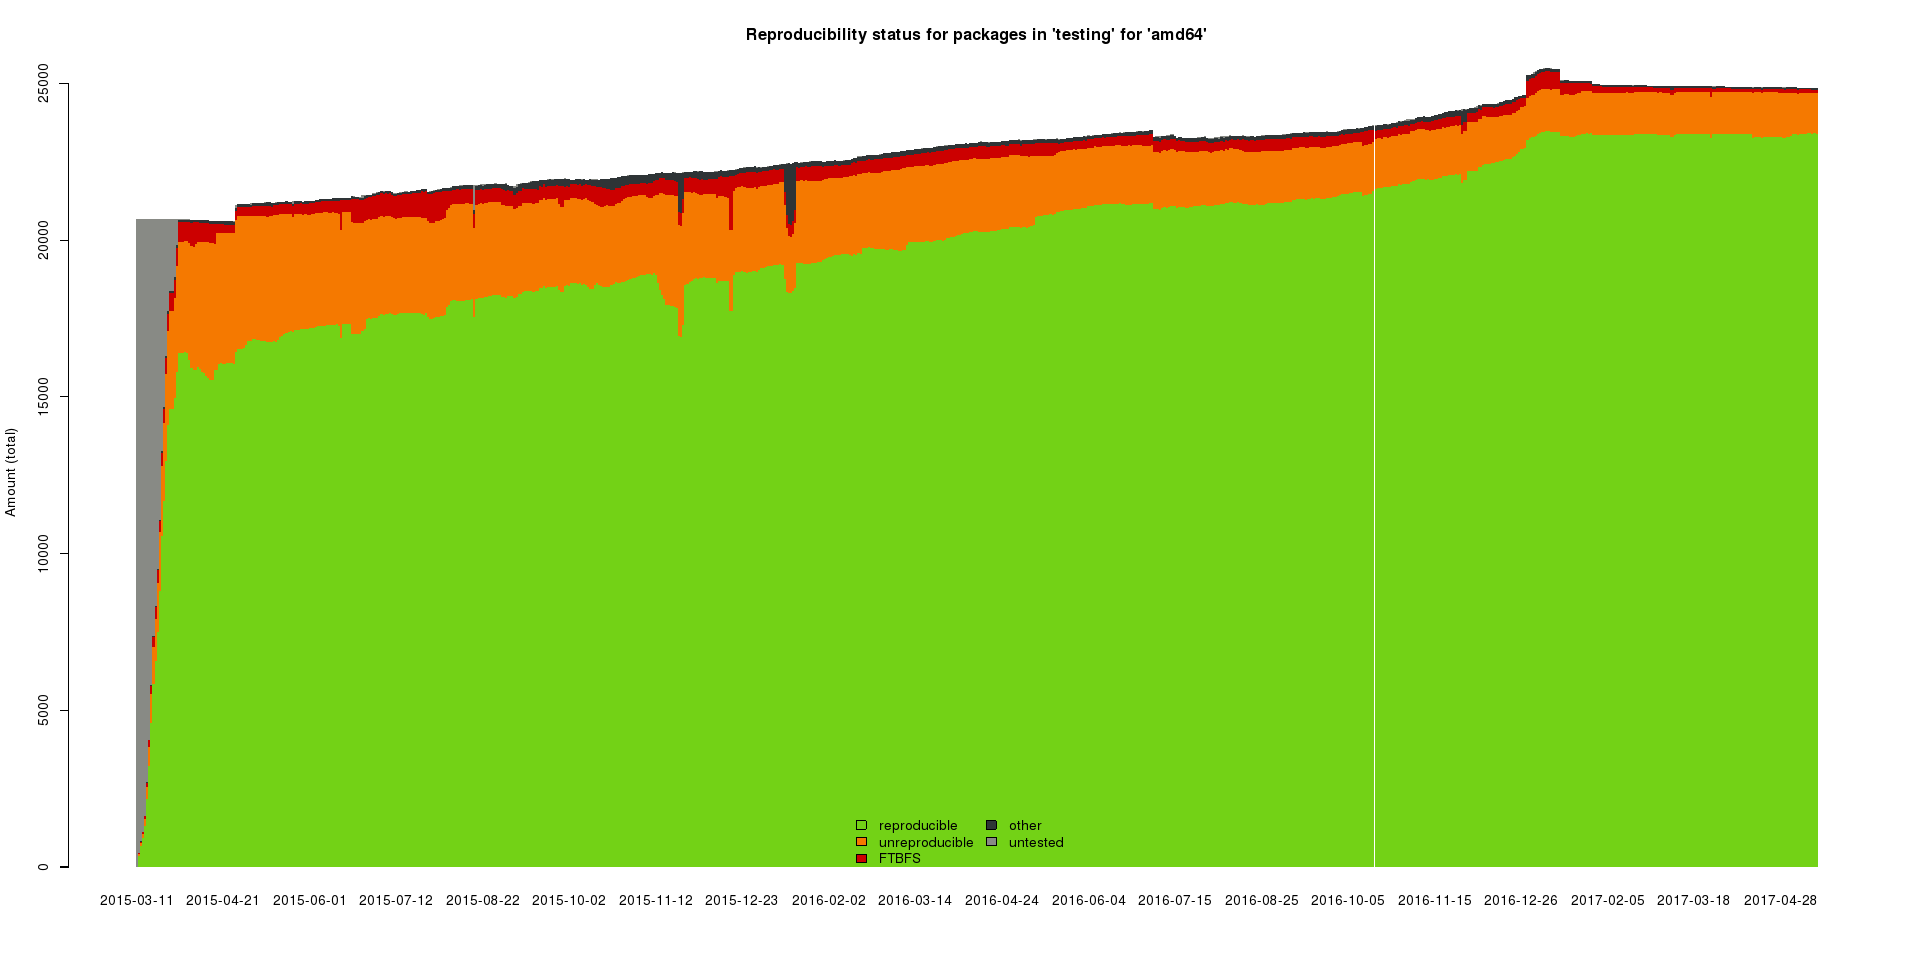
\includegraphics[width=0.95\textwidth]{fig/stats_pkg_state.png}
\caption{\label{fig:stats_sid}Overview of reproducible builds for packages in Debian unstable for amd64 architecture.}
\end{figure}

\subsubsection[Categorizing the issues]{Categorizing the issues} 
With diffoscope result for the packages available, Reproducible Builds project members try to identify the root issue causing reproducibility. It is often the case that the issue is not within the package itself, but rather in the tools used in the build process. Therefore, it is important to identify common issues and focus on resolving them in a unified way.\\\\
Some examples of the most common issues are:
\begin{itemize}[noitemsep]
\item \textit{Capturing build path} -- a lot of packages store the path where the package was built, during the build phase. This is inconvenient since this information is rarely helpful to end users; usually, the package is built on some dedicated build server and not on target computer. This issue is one of the main focus of Reproducible Build project members now, and they coordinate with maintainers of packages as well as build tools developers in order to address it.
\item \textit{Storing Timestamps} -- while this issue was addressed by \texttt{SOURCE\_DATE\_EPOCH}, some packages still record the build date or time.
\end{itemize}
Figure \ref{fig:stats_issues} illustrates the changes in the number of identified issues. This number generally rises over time, as new issues are being found and the old ones are often categorized into smaller and more specific issues. Even if the issue is completely dealt with, it is often left in records if it is believed information about it could be useful to other issues or other projects.\\\\

\begin{figure}
\centering
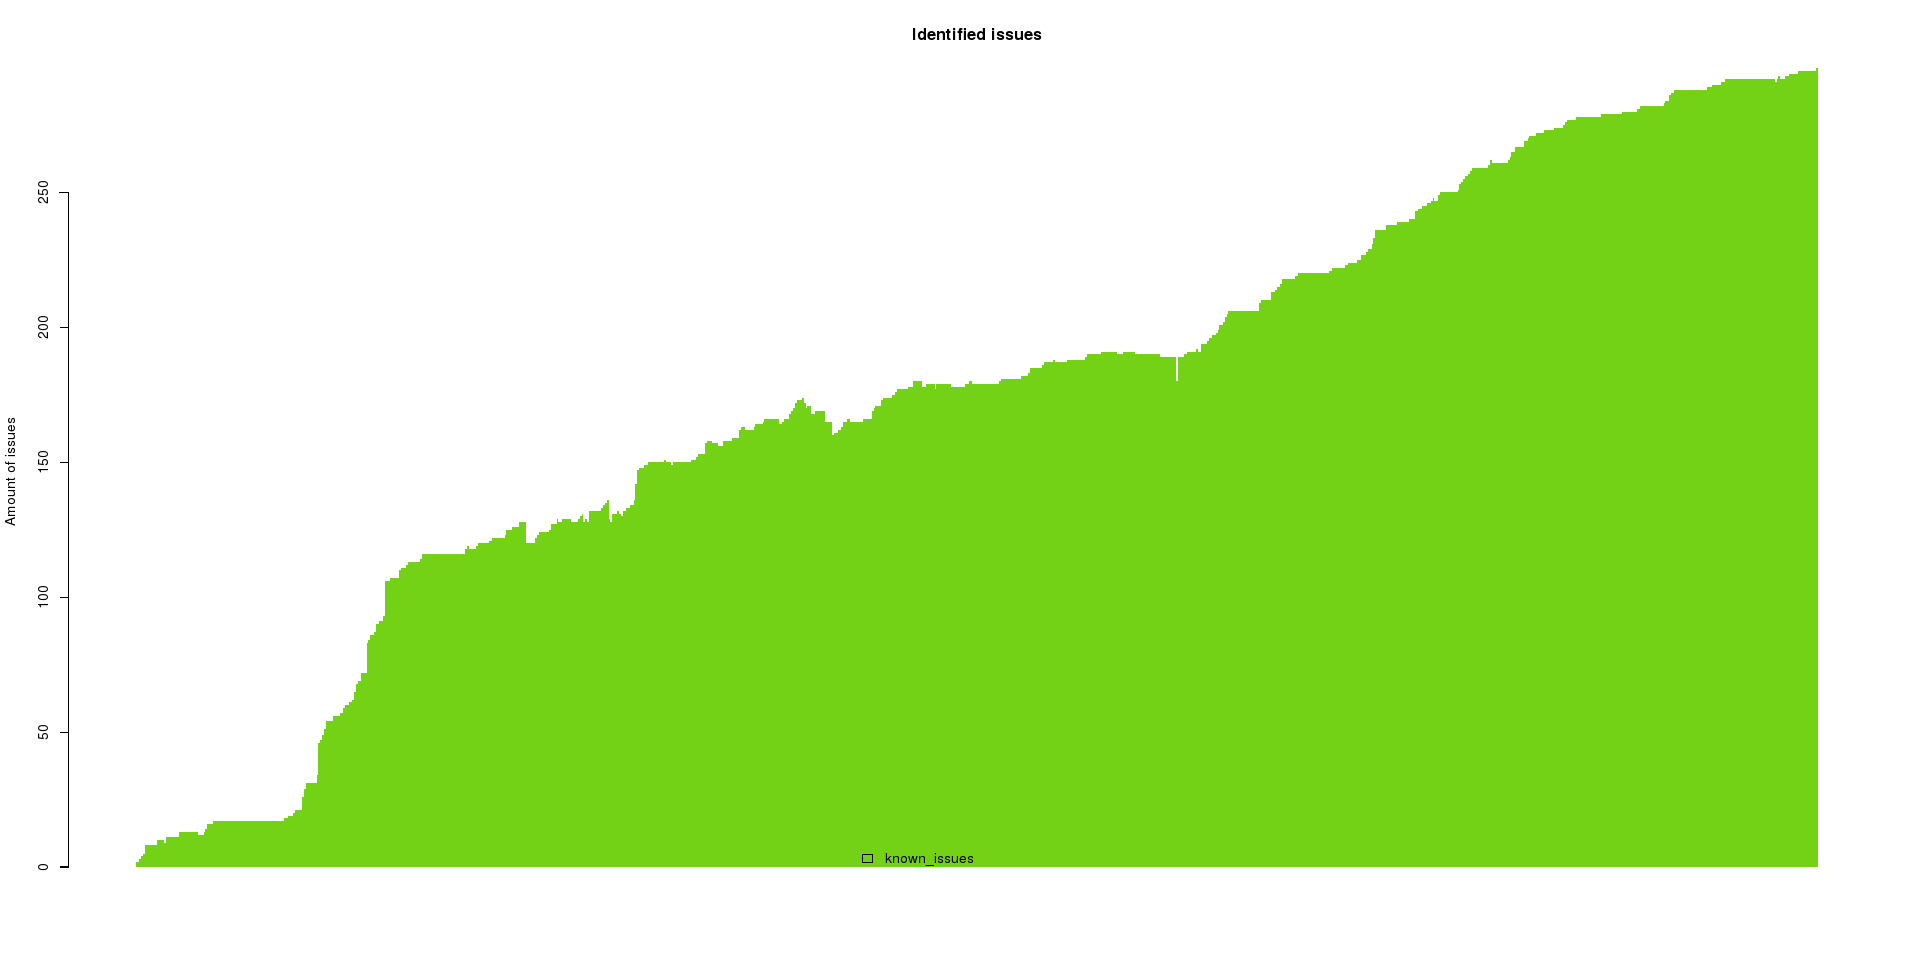
\includegraphics[width=0.95\textwidth]{fig/stats_issues.png}
\caption{\label{fig:stats_issues}Number of categorized reproducibility issues.}
\end{figure}

Figure \ref{fig:stats_notes} shows statistics about number of packages with notes attached to them, meaning that there is an identified issue or some sort of comment for them attached to them. Once again, a massive change is observed at around August, 2016, as the build path variation was introduced, resulting in a lot of packages being labeled with build path recording issue.\\

\begin{figure}
\centering
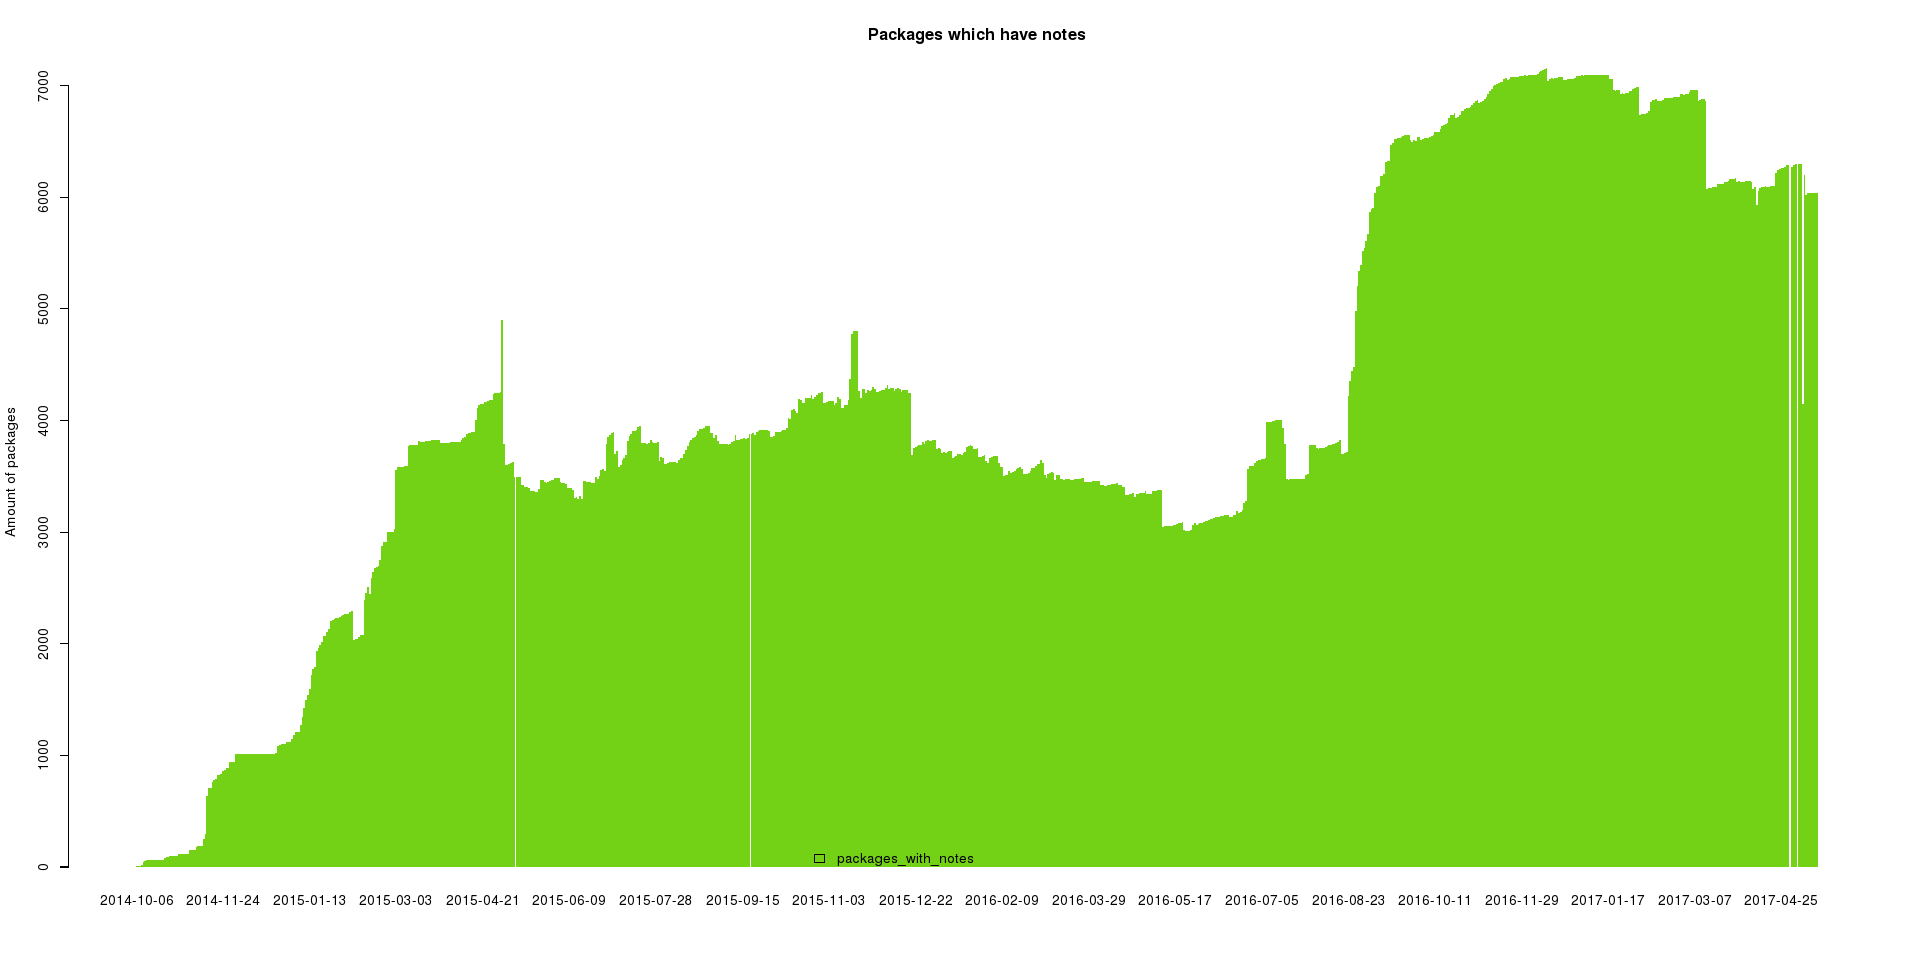
\includegraphics[width=0.95\textwidth]{fig/stats_notes.png}
\caption{\label{fig:stats_notes}Number of packages that have notes.}
\end{figure}
\subsubsection[Fixing reproducibility bugs]{Fixing reproducibility bugs}
While only package maintainers or developers actually have the means to fix their package, members of Reproducible Builds project try to help them by reporting the reproducibility issue. As a rule, they also provide a patch that is expected to fix the issue. Sometimes additional coordination with package maintainer or developer is required to ensure the patch fits well within the package and to clarify its meaning.\\\\
A lot of issues are related to the usage of the specific tool in the build process, and therefore it is usually preferred to focus on fixing these issues in the build tool in question, therefore helping all the packages using that tool to achieve reproducibility.

}
\subsection[F-droid]{F-droid}
\nopagebreak[4]{
The F-Droid project \autocite{fdroid}, that aims to provide an environment of free software for Android smartphones, has set up its own Verification Server \autocite{fdroid-vfs}. It functions in the similar fashion as Debian test infrastructure, rebuilding packages and providing the diffoscope output when results do not match.\\
}
\subsection[Other projects]{Other projects}
\nopagebreak[4]{
FreeBSD and NetBSD distributions also continue their work on reproducible builds. Currently, they use less variations between builds than Debian does, but within these constraint, they have achieved significant progress: NetBSD reported 100\% reproducibility within their build system in \autocite{netBSD} and FreeBSD is at 99.6\% at the moment \autocite{freeBSD}.
}


%\cleardoublepage
 %Current state of the project
\section{Conclusions}
\nopagebreak[4]{
  Reproducibility of software builds is important problem, critical for
  ensuring quality and security of open-source software. With the software
  building reproducibly, users can easily ensure no flaws were added to
  the product during build process and that the software indeed matches its
  source code. This problem attracted attention in various open-source projects,
  but outside of open-source world it is still not discussed enough. \\\\
  In this report, the history and motivation behind the
  Reproducible Builds project was presented. The definition of reproducibility
  in the software building process was given. An overview on the current reproducibility status of Debian operating system, as well as the steps taken to improve it, was discussed. Specifically discussed were the tools that the
  Reproducible Build project uses for testing reproducibility of software and
  identifying sources of unreproducibility. The particular tool for comparing
  two build outputs, named diffoscope, was discussed in detail, with emphasis on
  what can be done to improve it.
}

%\cleardoublepage
 %Conclusions

%\def\refname{what ever}% to change References title
\addcontentsline{toc}{section}{References}%

%\bibliography{ref}%
%\bibliographystyle{LUTapa}%
%\bibliographystyle{abbrv}
\printbibliography

%\cleardoublepage %

\end{document}
